\subsection{Results}

\begin{figure}[H]
    \centering
    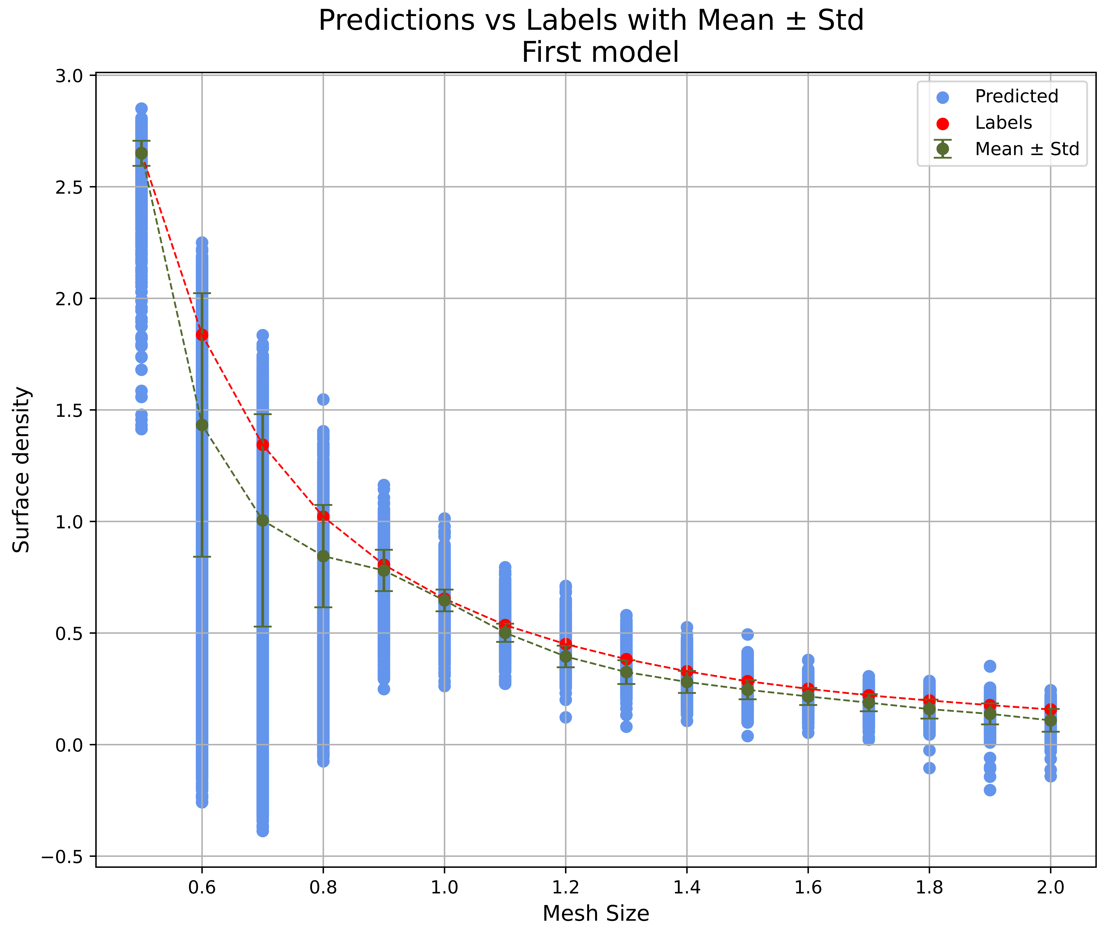
\includegraphics[width=0.5\textwidth]{figures/predict_vs_label_first_lowQ.png}
    \caption{Predicted surface densities vs truth label. Model trained on 0.5, 1.0 and 2.0 mm meshsizes}\label{fig:pred_vs_label_first}
\end{figure}

\begin{figure}[H]
    \centering
    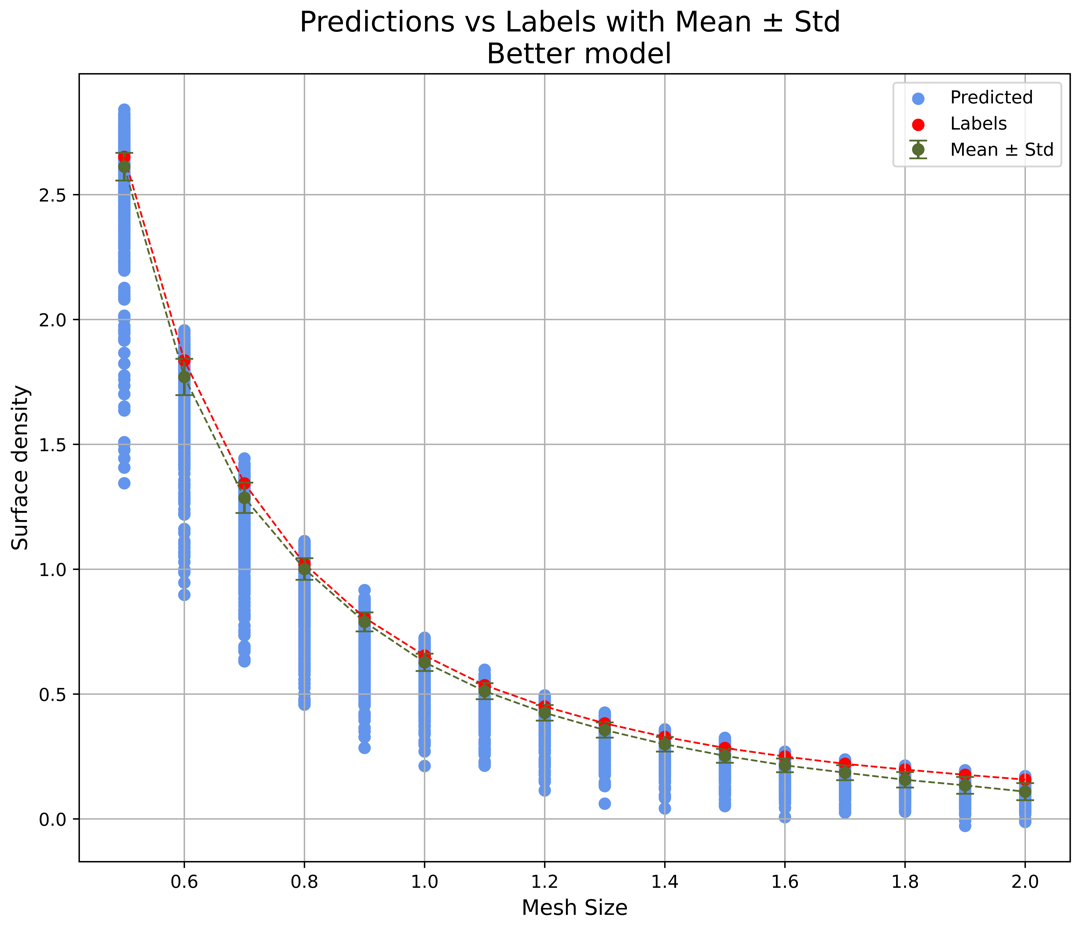
\includegraphics[width=0.5\textwidth]{figures/predict_vs_label_better_lowQ.png}
    \caption{Predicted surface densities vs truth label. Model trained on 0.5 to 2.0 mm meshsizes with 0.1 mm intevals}
    \label{fig:pred_vs_label_better}
\end{figure}

\begin{figure*}[t]
    \centering
    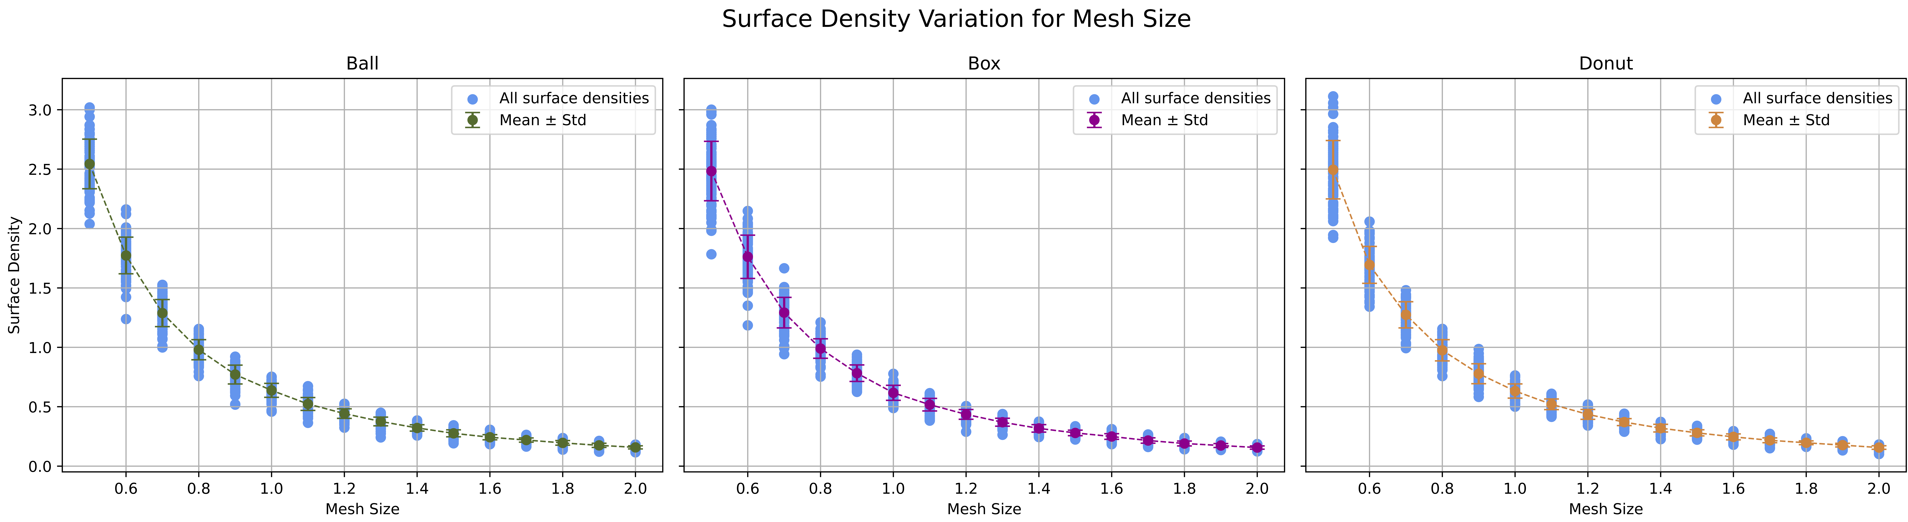
\includegraphics[width=\textwidth]{figures/sd_vs_mesh_lowQ.png}
    \caption{Variation in surface density for different shapes at different meshsizes}
    \label{fig:sd_mesh}
\end{figure*}

\begin{figure*}[t]
    \centering
    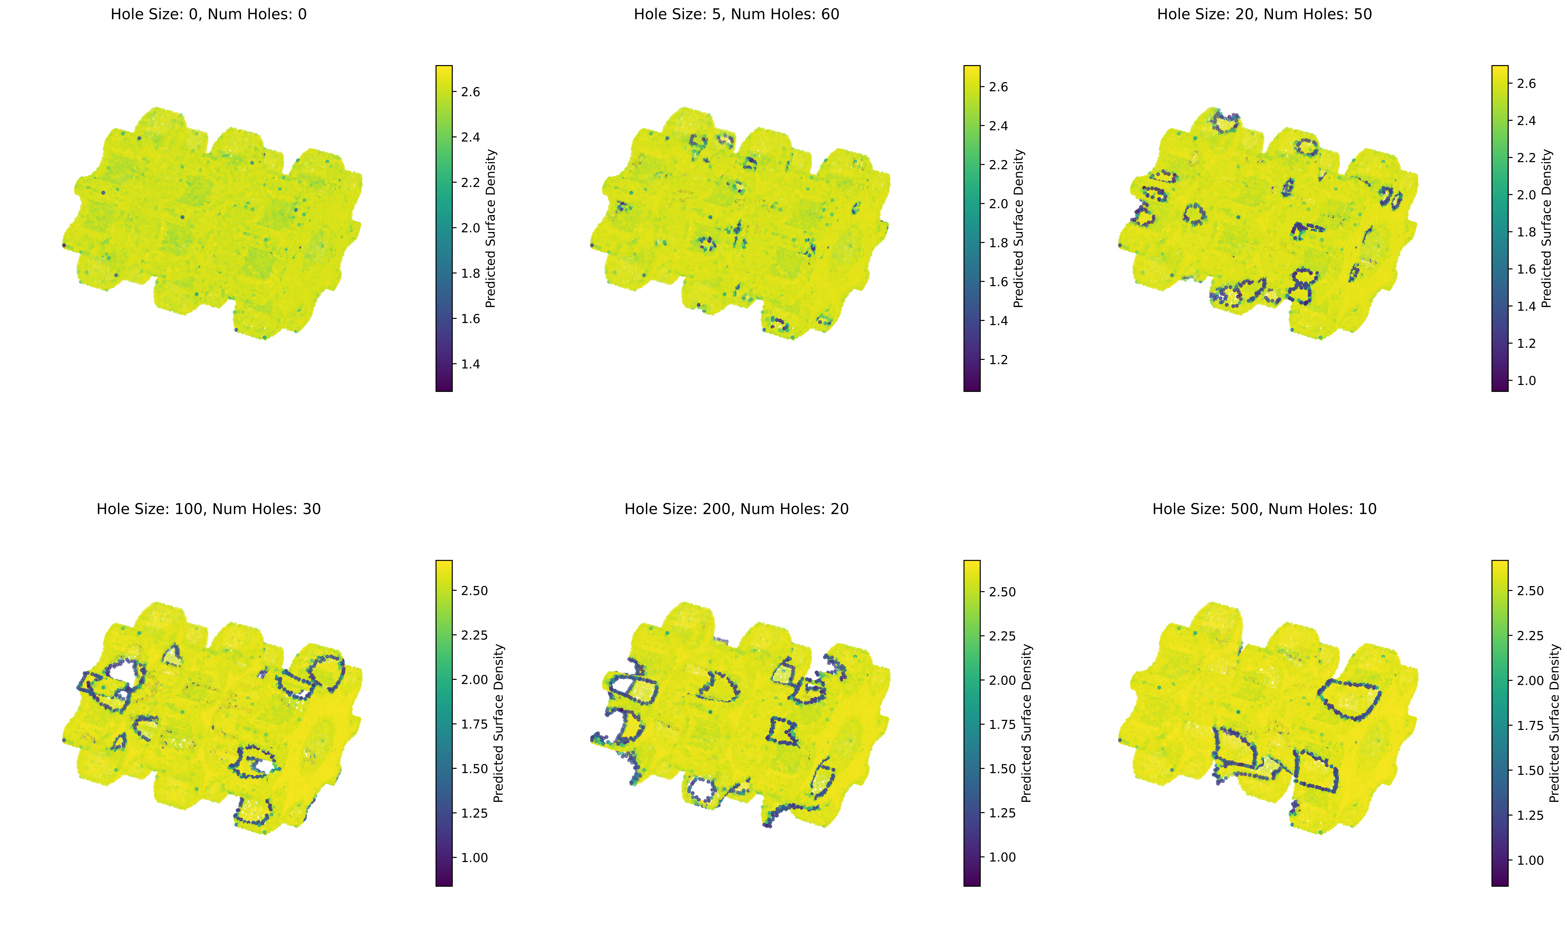
\includegraphics[width=\textwidth]{figures/result3_lowQ.png}
    \caption{Surface density predictions for the same pointcloud with varying holesizes.}
    \label{fig:holes_predict}
\end{figure*}

\begin{figure}[H]
    \centering
    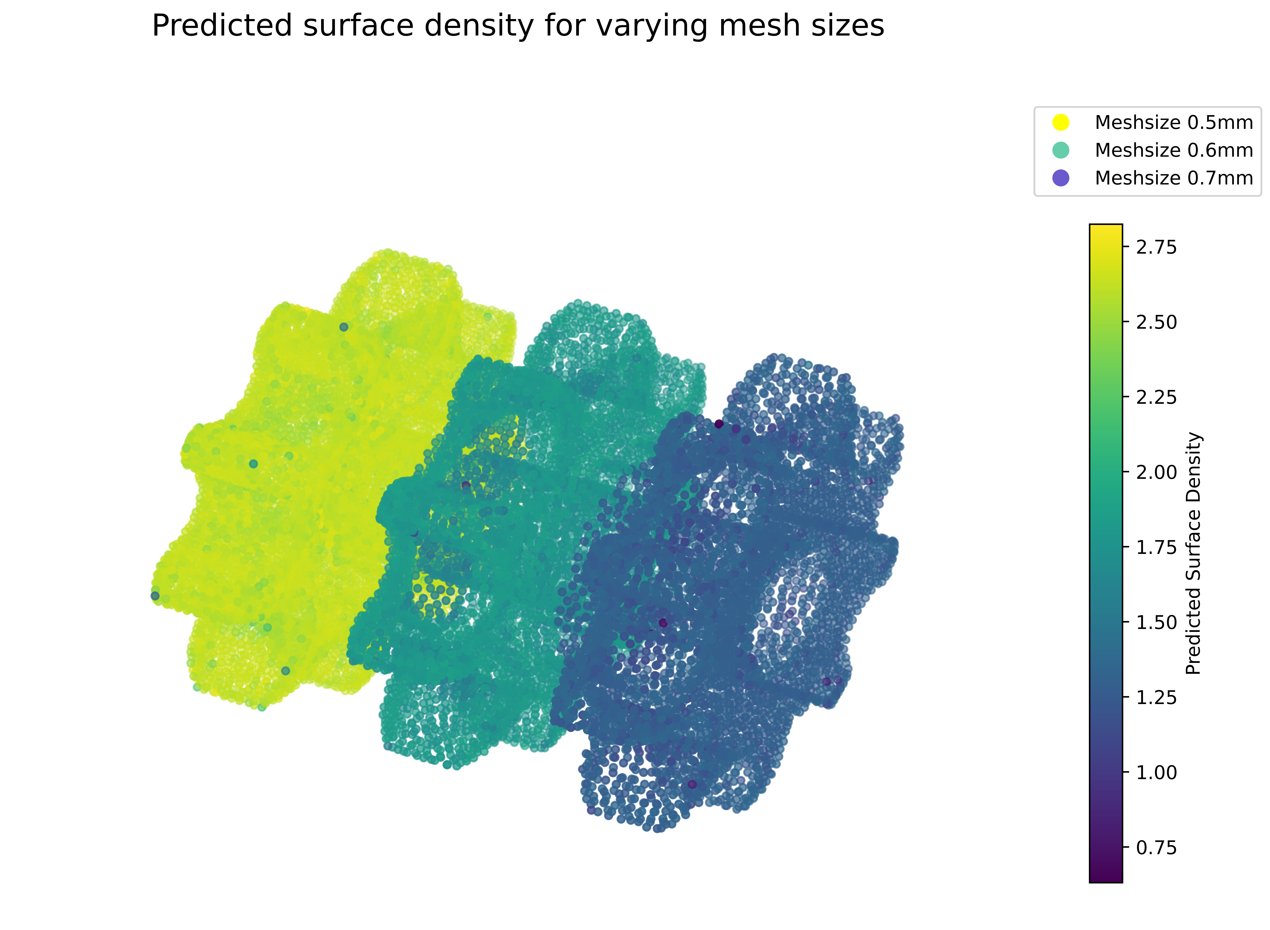
\includegraphics[width=0.5\textwidth]{figures/varying_meshsize_lowQ.png}
    \caption{Surface density predictions for meshsizes: 0.5, 0.6 and 0.7}
    \label{fig:diff_mesh_predict}
\end{figure}
